\documentclass[11pt]{article}
\usepackage[toc,page]{appendix}
\usepackage{amsmath, amssymb}
\usepackage[utf8]{inputenc}
\usepackage[T1]{fontenc}
\usepackage[style=apa,backend=biber]{biblatex}
%\usepackage{biblatex}
\addbibresource{references.bib}
\usepackage{graphicx}
\usepackage{tikz}
\usetikzlibrary{automata,positioning,shapes.geometric, arrows.meta, fit, backgrounds, calc, chains}
\graphicspath{./images/Easy_Pictures/SMR_MULT_Repackaging}%\usepackage{kpfonts}
\usepackage{float}
\usepackage[margin=1in]{geometry}
\usepackage{cancel}
\usepackage{epsfig}
\usepackage{tikz-3dplot}
\usepackage{darkmode}
\usepackage{dirtytalk}
\usepackage{longtable,booktabs,array}
\usepackage{calc} % for calculating minipage widths
\usepackage[utf8]{inputenc}
\usepackage[T1]{fontenc}
\usepackage{xcolor}
\usepackage{listings}


\usepackage{etoolbox}
\usepackage{hyperref}
\hypersetup{
 colorlinks=true,
 linkcolor=blue,
 filecolor=magenta, 
 urlcolor=cyan,
 pdftitle={Hermeneutic Calculator},
 citecolor=blue,
 }


\urlstyle{same}

\lstdefinestyle{htmlStyle}{
 language=HTML,
 basicstyle=\ttfamily\small,
 keywordstyle=\color{blue}\bfseries,
 commentstyle=\color{gray}\itshape,
 stringstyle=\color{red},
 breaklines=true,
 frame=single,
 numbers=left,
 numberstyle=\tiny\color{gray},
 columns=fullflexible,
}
\lstdefinelanguage{HTML}{
 keywords={<!DOCTYPE, html, head, title, body, h1, h2, h3, p, div, span, a, img, ul, li, table, tr, td, th, style, link, script},
 sensitive=true,
 comment=[l]{//},
 morecomment=[s]{/*}{*/},
 morestring=[b]',
 morestring=[b]"
}
\lstset{style=htmlstyle, language=html}
% Updated to explicitly pass the language option
%\lstinputlisting[style=htmlstyle, language=html]{./html/example.html}
%\usepackage{tocloft}

% Optional: define some custom colors
\definecolor{sliceRed}{RGB}{225,224,91} % matching "varyellow" from your code
\definecolor{linkYellow}{RGB}{255,215,0} % a golden yellow
\tdplotsetmaincoords{70}{110}

\title{Subtraction Strategies: Counting On/Back By Bases and then Ones (CBBO)}
\author{Compiled by: Theodore M. Savich}


\begin{document}
\maketitle
\subsection*{Transcript}
Video from \textcite{Carpenter1999}. Strategy descriptions and examples adapted from \textcite{HackenbergCourseNotes}. 
\begin{itemize}
\item \textbf{Teacher:} Earl had a collection of 65 bird feathers, on a trip to a marsh he found lots more feathers to put in his collection. Now he has 94 feathers in his collection. How many feathers did Earl find at the marsh? 
\item \textbf{Rita} So he had what? 
\item \textbf{Teacher:} He started off with, 65 feathers. 
\item \textbf{Rita:} 1,2,3,4,5,6 1,2,3,4,5. And then he had how many? 
\item \textbf{Teacher:} Well, he had 65 bird feathers. On a trip to a marsh, he found lots more and he put them in his collection. Now he has 94. 
\item \textbf{Rita:} Well, I can 65, 75, 85. How many did he find? 
\item \textbf{Teacher:} Well, that's my question for you. How many did he find? He ends up with 94. 
\item \textbf{Rita:} And 85,86,87,88,89,90, 91,92,93,94 and so the answer is 20, 21, 22, 23, 24, 25, 26, 27, 28, 29. 
\item \textbf{Teacher} Nice work.

\end{itemize}

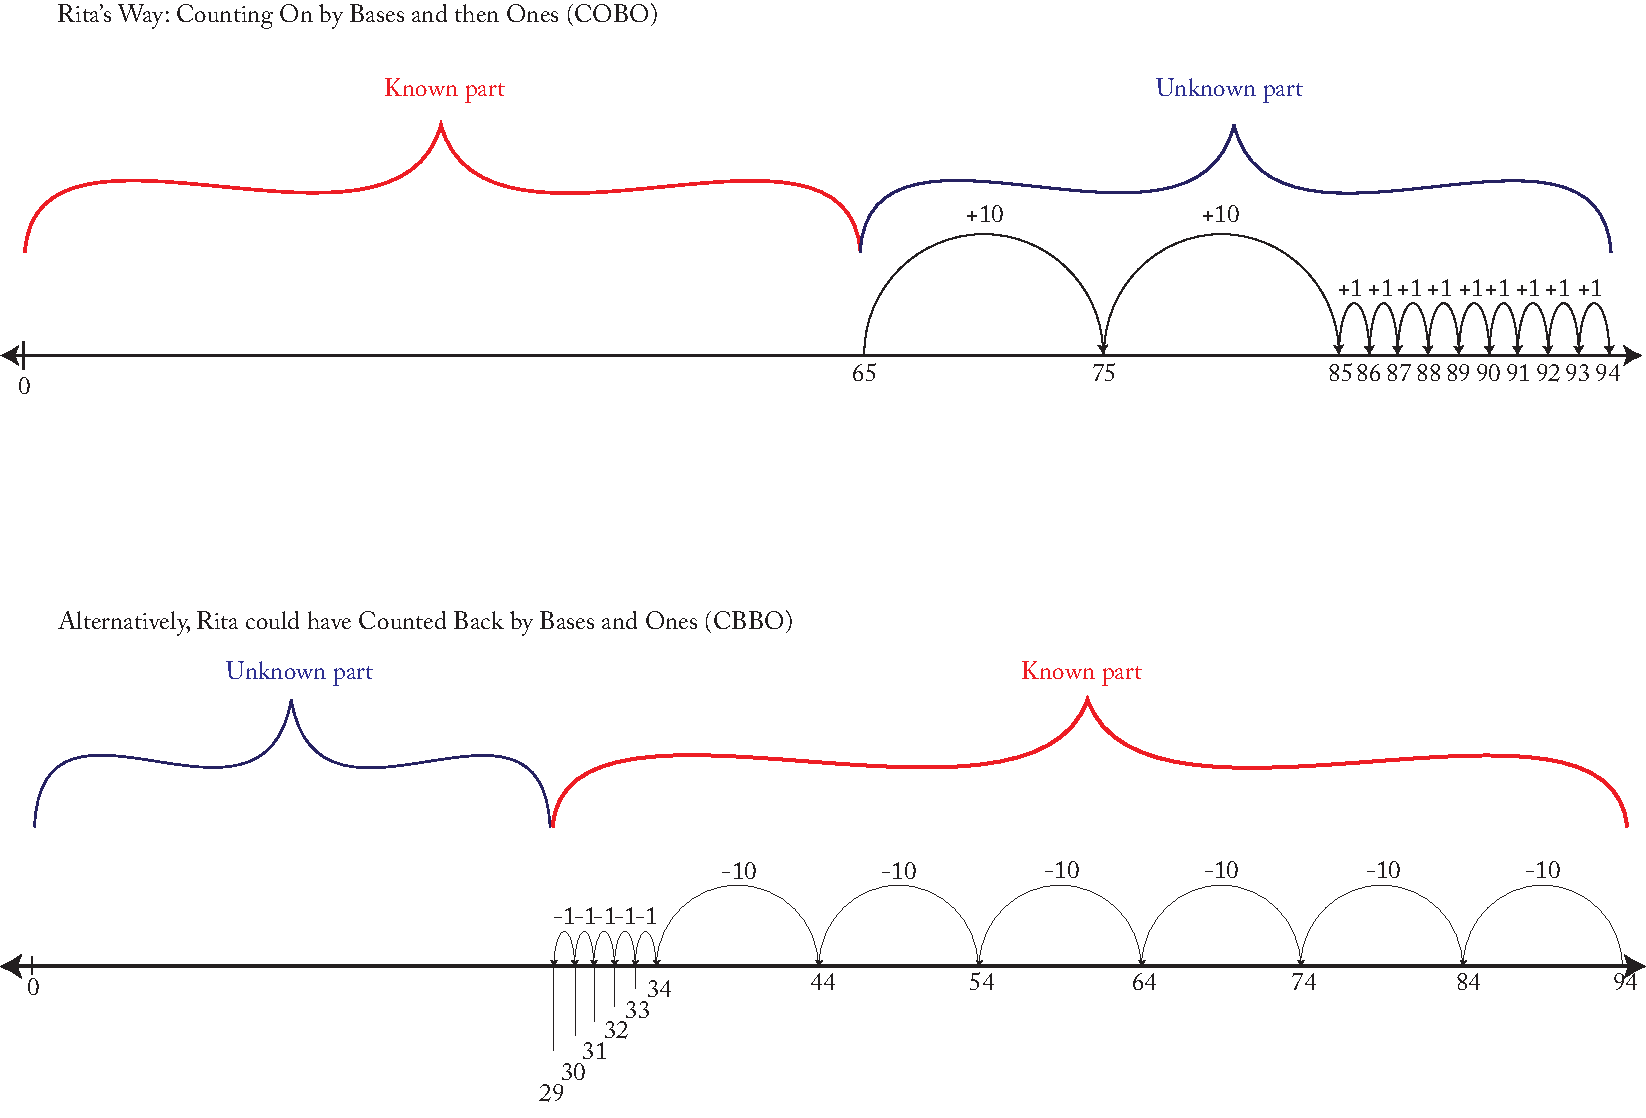
\includegraphics[width=.8\textwidth]{images/Easy_Pictures/SAR_SUB_COBO/PDF/SAR_SUB_COBO_CBBO.pdf}

\noindent \textbf{Notation Representing Rita's Solution:}
\begin{align*}
    65 + (10) &= 75\\
    75 + (10) &= 85\\
    85 + 1 + 1 + 1 + 1 + 1 + 1 + 1 + 1 + 1 &= 94\\
    10 + 10 + 1 + 1 + 1 + 1 + 1 + 1 + 1 + 1 + 1 &= 29
    \end{align*}
    

\subsubsection*{Description of Strategy:}

 \textbf{Objective:} Description of Counting On by Bases and Then Ones (COBO)
 Begin with one of the numbers. Break the other number into its base units and its ones. Then, “count on” by adding each base unit one at a time, followed by each individual one.
 
 Why are number lines useful for demonstrating this strategy?
 COBO is essentially a jump strategy—you start at one number and make “jumps” equal to the other number’s base units, then add in the remaining ones. Number lines are ideal because they visually display jumps of varying lengths and directions. They serve as a picture of the process: a jump representing a full base is clearly larger (by a factor of the base) than a jump of a single unit.
 
 Good number line illustrations should:
\begin{itemize}
 \item Clearly represent the relative sizes of the jumps—each base jump should be exactly as many times larger than a single-unit jump as the base indicates, with all base jumps the same size and all one-unit jumps identical.
 \item Indicate the position of 0, or mark a break if that portion of the line isn’t drawn to scale.
 \item Use arrows to indicate direction—when adding, the jumps go to the right (or upward); when subtracting, they go to the left (or downward).
 \item Mark all landing points clearly—the numbers you would speak aloud when counting on by bases and then ones, just as Lauren demonstrated.
\end{itemize}

\subsubsection*{Automaton Diagram for Counting On or Back by Bases and Then Ones}

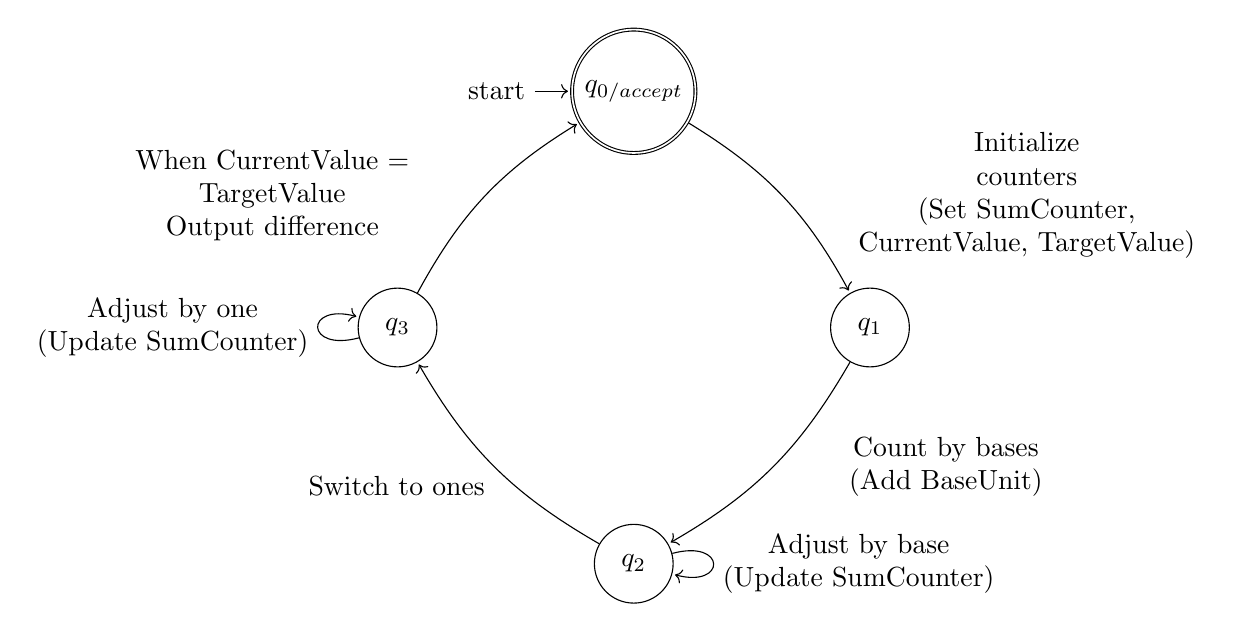
\begin{tikzpicture}[
 shorten >=1pt,
 auto,
 node distance=3cm,
 every state/.style={minimum size=1cm}
]
 % Arrange 4 states on a circle:
 % q_{0/accept} at 90°, q_1 at 0°, q_2 at 270°, q_3 at 180°.
 \node[state, initial, accepting] (q0) at (90:3cm) {$q_{0/accept}$};
 \node[state] (q1) at (0:3cm) {$q_1$};
 \node[state] (q2) at (270:3cm) {$q_2$};
 \node[state] (q3) at (180:3cm) {$q_3$};

 % Transition from q0 to q1: Initialize counters
 \path[->]
 (q0) edge[bend left=15] node[right=24pt, align=center] {Initialize\\counters\\(Set SumCounter,\\CurrentValue, TargetValue)} (q1)
 % Transition from q1 to q2: Count by bases
 (q1) edge[bend left=15] node[right=24pt, align=center] {Count by bases\\(Add BaseUnit)} (q2)
 % Loop on q2: Adjust by base if needed
 (q2) edge[loop right, looseness=7] node[right, align=center] {Adjust by base\\(Update SumCounter)} (q2)
 % Transition from q2 to q3: Switch to ones
 (q2) edge[bend left=15] node[below left, align=center] {Switch to ones} (q3)
 % Loop on q3: Count by ones
 (q3) edge[loop left, looseness=7] node[left, align=center] {Adjust by one \\ (Update SumCounter)} (q3)
 % Transition from q3 to q0: Output difference
 (q3) edge[bend left=15] node[left=24pt, align=center] {When CurrentValue = \\ TargetValue\\Output difference} (q0);
\end{tikzpicture}

\clearpage





\subsubsection*{HTML Implementation}
\lstinputlisting[style=htmlStyle, language=html]{./new_html/SAR_SUB_COBO.html}

\printbibliography
\end{document}